\newpage
\section {Subject-Phase Model based process specifications}

\subsection{Introduction}

There are different stakeholders in business process management (see e.g. in \cite{art:Stakeholder}, \cite{book:Worklow-Mod}, \cite{book:BPM-Handbook2}). The most important ones are the customers interested in the result of a process, managers responsible for processes (often called process owners) and the parties involved in the execution of a process (Providers). The parties involved in the execution of a process (providers) can be represented by subjects (see \cite{book:flei2011}. Subjects are abstract representations of the active elements in a process which communicate with each other in order to coordinate their work producing the required result of a process. Especially middle management wants to get an overview about the process from the event causing the execution of a corresponding process instance (e.g. subject representing the customer of a process) till the results of a process are delivered to the parties expecting it. In the most abstract way, upper management is only interested in Key Performance Indicators expressing the efficiency and effectiveness of a process. May be that the delivery of a process result causes the execution of a succeeding process. These succeeding processes use results of the proceeding process as input.
Middle management is interested in who is involved in a process and what  is their contribution to the process result and what are the cost for each contribution. Managers are not mainly interested in the details how the parties involved in a process execute their tasks, how they communicate with each other in order to coordinate their work and which tools and means they use to do their work. Whereas the parties involved in the execution of a process are exactly interested in these aspects of a process. The parties involved in the execution of a process want to know what work they have to do, in which sequences they have to execute these tasks, including when they have to communicate with whom about what and last but not least which means they use for doing their tasks.
On the one hand processes have to be described precisely enough that the parties involved in a process execution know what they have to do in which situation and on the other hand management is primarily interested in more abstract process attributes like key performance indicators and the structure of a process, depending on the management level.\\

Additionally abstract views on processes are needed if complex process systems have to be defined and a top down approach for describing processes is applied. First designers create an overview of a process system and then this abstract model is refined step by step till a model is created which is good enough for the parties working in a process. In order to define hierarchically most methods and tools for process management use different approaches to solve that problem.
In that article an approach is described which allows to get an overview of the involved parties of a process and what are their major contributions to the result of a process. Practical experience show that this approach allows to describe the dynamic os a process on one page and the specification is precisely enough to derive executable workflows.

\subsection{Related Work}

Many approaches exist in order to express hierarchies of processes in business process management. In general three to five levels of process specification are used (e.g. see page 53 in \cite{book:Worklow-Mod}, page 52 in \cite{book:Prozessmgmt-umsetzen}, page 92 in \cite{book:EnterpriseBPM}) These process levels are mainly called process areas, business processes, processes, sub-processes and activities. Sometimes sometimes business processes are classified in kernel processes, and main processes (see \cite{book:EnterpriseBPM} page 87. 
In the following sections the abstraction concepts in the mostly used process modeling approaches are outlined.\\

In the ARIS (see \cite{book:ARIS}, \cite{book:SAPRoadmap}, \cite{book:EnterpriseBPM}) ecosystem process chains are used in order to give an overview of a process. A process chain shows the process of a process system and defines the sequence in which these processes in the process system can be executed.  There can be several levels of process chains. This means an element representing a process of a process chain can also contain a process chain and so on.  In the lowest level each element of a process chain contains a Event driven Process Chain (EPC). The event driven process chain contains the activities executed in a process. On EPC level the activities are connected to subjects who have to execute an activity. This means only at the lowest level a manager can see who is involved in the execution of a process. It is possible that an activity in an EPC is not one single activity. It can again be an EPC. These various levels of abstraction are focused on the activities executed in a process.\\

BPMN has pools and swim lanes for describing process structures (see \cite{Standard:BPMN}). A process consists of one or several pools and each pool can consist of one or several swim lanes. It is not allowed to have pools in a pool or swim lanes in a swim lane. Activities are assigned to swim lanes. This means there are three abstraction layers: Pools, Swim Lanes and Activities. Pools and swim lanes are used to structure the activities in a process. An activity can contain a sequence of activities. This activity type is called subprocess. An activity in a subprocess can also be a subprocess and so on. This means on activity level arbitrary levels of subprocess are possible. In subprocesses pools and swim lanes are not allowed. Each activity is assigned to a party executing that activity. This means that a pool or swim lane does not correspond to a certain doer. Each activity in a swim lane can be executed by a different provider.\\

This two ways of abstraction are similar to the abstraction used in control flow charts. Only at the lowest level management can see who is involved in a process. The other way around the parties executing the actions have to scan through all the activity sequences in order to find the actions which they have to execute. 
\\
In this paper I want to show an approach in order to specify processes on different abstraction levels for the major stakeholders: Management and doer or provider. On one page managers and the actors in a process see the structure of a process (people and activities) and they get an overview who has to execute which action when.


\subsection{Subject Phase Matrix (S-PM)}

The features of the subject phase matrix will be demonstrated with an example from a real process management project in a small transport company. Figure \ref{fig:process-arch} shows part of the process architecture of that company. There are three processes which built a process chain. There is the process 'Order'. In that process the order of customer will be checked and the transport will be prepared. In process 'Transport' the goods will be transported and in process 'invoicing' the message 'invoice' is send to the subject 'customer' and its payment is controlled. 

\begin{figure}[hbtp]
	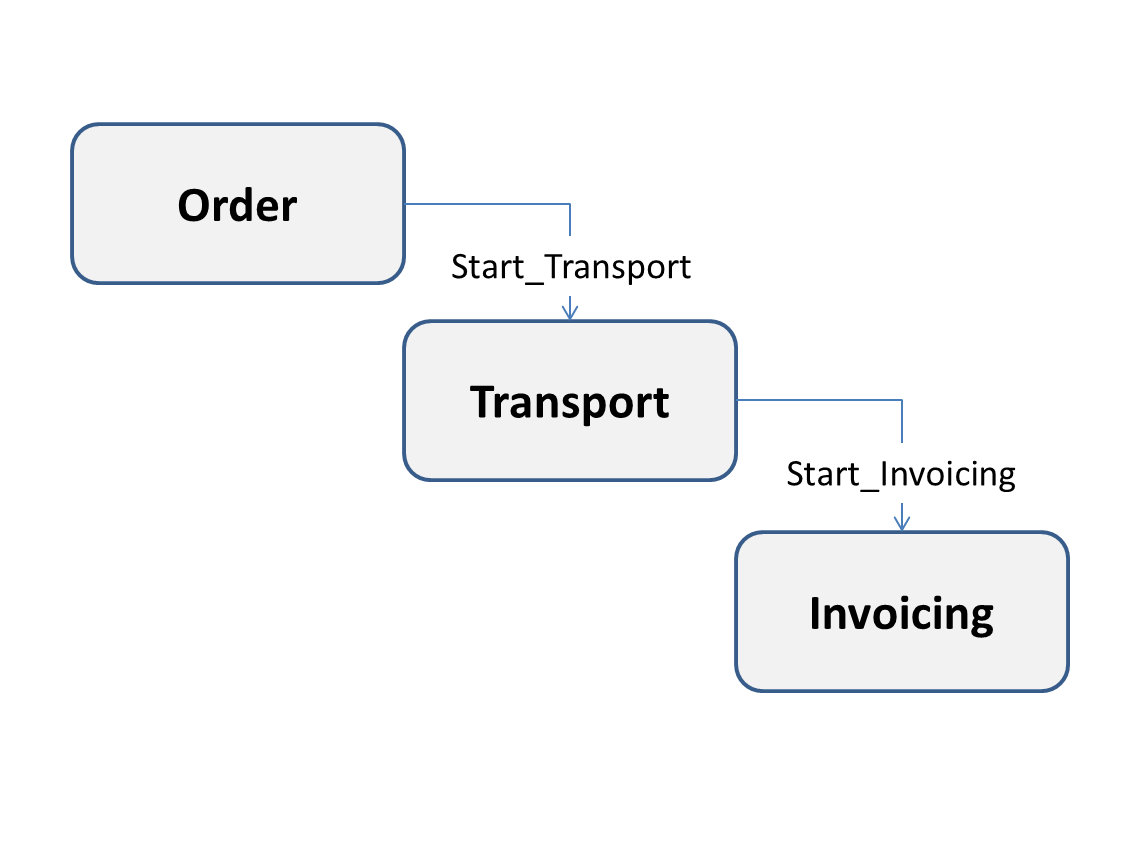
\includegraphics[scale=0.2]{Figures/Chapter5/Subject-Phase/process-architecture.png}
	\caption{Process-architecture}
	\label{fig:process-arch}
\end{figure}

The execution logic of each of these processes is described with a subject-phase matrics (S-PM). The following figure \ref{fig:S-PM-Order} shows the S-PM of the process order.

\begin{figure}[hbtp]
	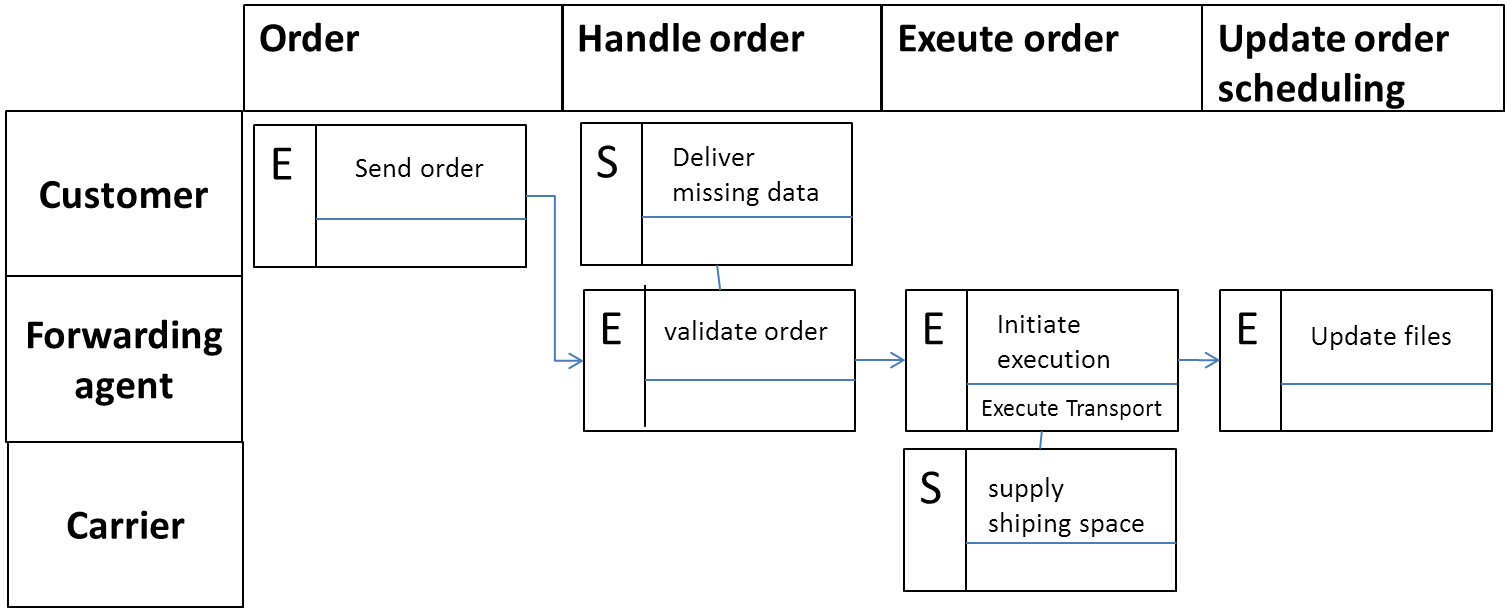
\includegraphics[scale=0.2]{Figures/Chapter5/Subject-Phase/S-PM-process-Ortder.png}
	\caption{S-PM of process 'Order'}
	\label{fig:S-PM-Order}
\end{figure}

A S-PM shows the subjects of a process in the most left column. Subjects  represent the acting parties in a process. Subjects are abstract resources like in S-BPM (see \cite{book:flei2011}). The subjects in Figure \ref{fig:S-PM-Order} are 'customer', 'forwarding agent' and 'carrier'. An S-PM does not show the embedding of a process into an organization. This is a completely separate step as described in \cite{book:flei2011}. This means in that article only the process model is considered. The implementation activities are analog to S-BPM (as described in \cite{book:flei2011}).
Process 'order' shown in \ref{fig:S-PM-Order} has the phases 
\begin{itemize}
	\item order 
	\item handle order
	\item execute order
	\item update scheduling
\end{itemize}
A process is executed from the left to the right, but loops back to proceeding phases are allowed. This means a process starts with the most left phase. In the columns representing the various phases of a process the activities executed in that phase are specified. In a phase it is defined which subject executes which major activity set (marked by an E) and which subjects execute supporting activities (Marked by an S) for the executing subject. In figure \ref{fig:S-PM-Order} the subject 'Customer' executes the activity 'send order' in phase 'order'. In phase 'Handle order' the subject and 'Forwarding agent' are involved. The subject 'Forwarding agent' validates the order and the subject 'Customer' supports in that action. In order to get this support the subject 'Forwarding agent' communicates with the subject 'Customer'. In phase 'Execute order' the subject 'Forwarding agent' is supported by the carrier. In that phase subject 'Forwarding agent' starts the process 'Execute Transport' (Lower part of the rectangle representing the major activity in phase Execute order). If phase 'Execute Order' is finished subject 'Fprwarding Agent' executes in phase 'Update Order Schedulin' the activity 'Update Files'. Figure \ref{fig:S-PM-Execute-Trans} shows the S-PM of process 'Execute Transport' initiated in process 'Order' in phase 'Execute Order' by subject 'Forwarding Agent'.

\begin{figure}[hbtp]
	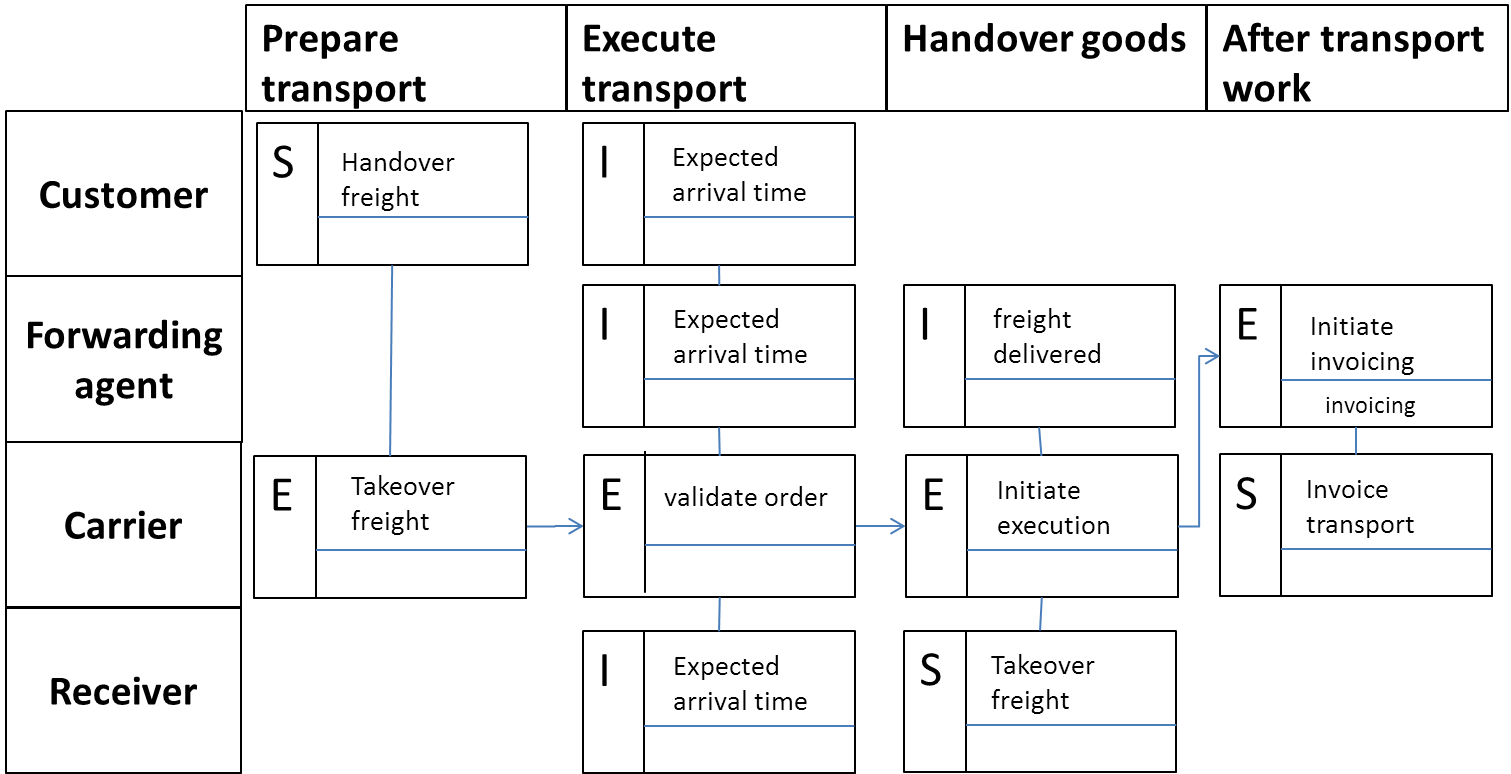
\includegraphics[scale=0.2]{Figures/Chapter5/Subject-Phase/execute-transport.png}
	\caption{S-PM of Process 'Execute Transport'}
	\label{fig:S-PM-Execute-Trans}
\end{figure}


In process 'Execute Transport' some activities are marked with an I. This means that the corresponding subjects are only informed. In phase 'Execute process' subject 'Carrier' informs the subjects 'Customer', 'Forwarding agent' and 'Receiver' about the 'Expected arrival time'.
\\
In the S-PM 'Execute Transport' there is also a subject named 'Customer'. This subject is different from the subject 'Customer' in the S-PM 'Order'. Subject names in a S-PM are valid in the corresponding process. This means subjects in different processes with the same name are different subjects. This does not mean that during the execution of a process (process instance) subjects with the same name in different processes are handled by different persons. Which providers (persons or machines) executes the activities of a subject are defined in the organisational embedding. This is not considered in that paper. This is a task of embedding subjects in an organization (see \cite{book:flei2011}).
\\
S-PMs give an overview about the subjects involved in a process, which activities they execute in which sequence and which relations exists between the various subjects. In many real projects (ISO 9001 projects) more than hundred processes have been specified in that way. It showed up that each process can be structured in phases and processes have between three and six phases only a small number (around 2 percent) have more than six phases. In all cases S-PMs did have more than one page. There has been also the experience that S-PMs are easy to understand also for management and gives the involved parties a first impression what they have to do in a process. In spite of their overview character S-PMs are precise enough that a S-BPM specification can be automatically derived. This will be shown in the following section.

\subsection{Conversion of Subject Phase Matrix to Subject Communication Models}
The conversion of the Subject-Phase-Matrix into Subject Communication Diagrams (SCD) and Subject Behavior Diagrams (SBC) can be done automatically (see \cite{book:flei2011}). In general these SCDs and CBCs are executable without any additionally programming (see \cite{book:flei2011}) but the business objects must be added manually and some internal activities must be specified in more detail. In the following the focus is on the behavior of subjects. Data or business objects are not considered.\\

In order to transform an S-PM into a subject-communication specification we consider the matrix from the perspective of the involved subjects (see figure \ref{fig:S-PM-Execute-Trans}).
\begin{figure}[hbtp]
	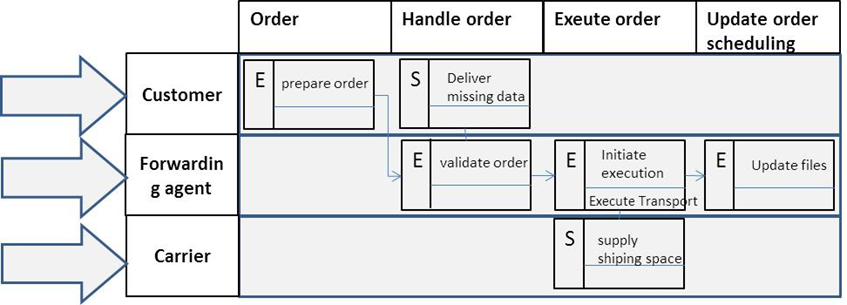
\includegraphics[scale=.4]{Figures/Chapter5/Subject-Phase/s-PM-subject-view.png}
	\caption{S-PM considered from the subject view}
	\label{fig:S-PM-subject-view}
\end{figure}
Each subject in the matrix corresponds to a subject in the subject communication diagram. The names of the subjects in the S-PM are extended with an Id for the process. In our case to each subject name the letters AO are added (AO=Accept Order). A subject sends a message to another subject if in the S-PM the E-action in the succeeding phase is executed by a different subject or the subject needs supports from an other subject. If subjects send a message to the subject executing the E-activity in the succeeding phase the message is named 'E-name-of the-succeeding-phase'. If a subject requests support from another subject the message is named 'S-Name-of-the-phase?'. The receiving subject sends the result of the support request back with a message called 'S-Name-of-the-phase!'. Figure \ref{fig:SCD-Order} shows the communication structure derived from the S-PM shown in figure \ref{fig:S-PM-Order}.
\begin{figure}[hbtp]
	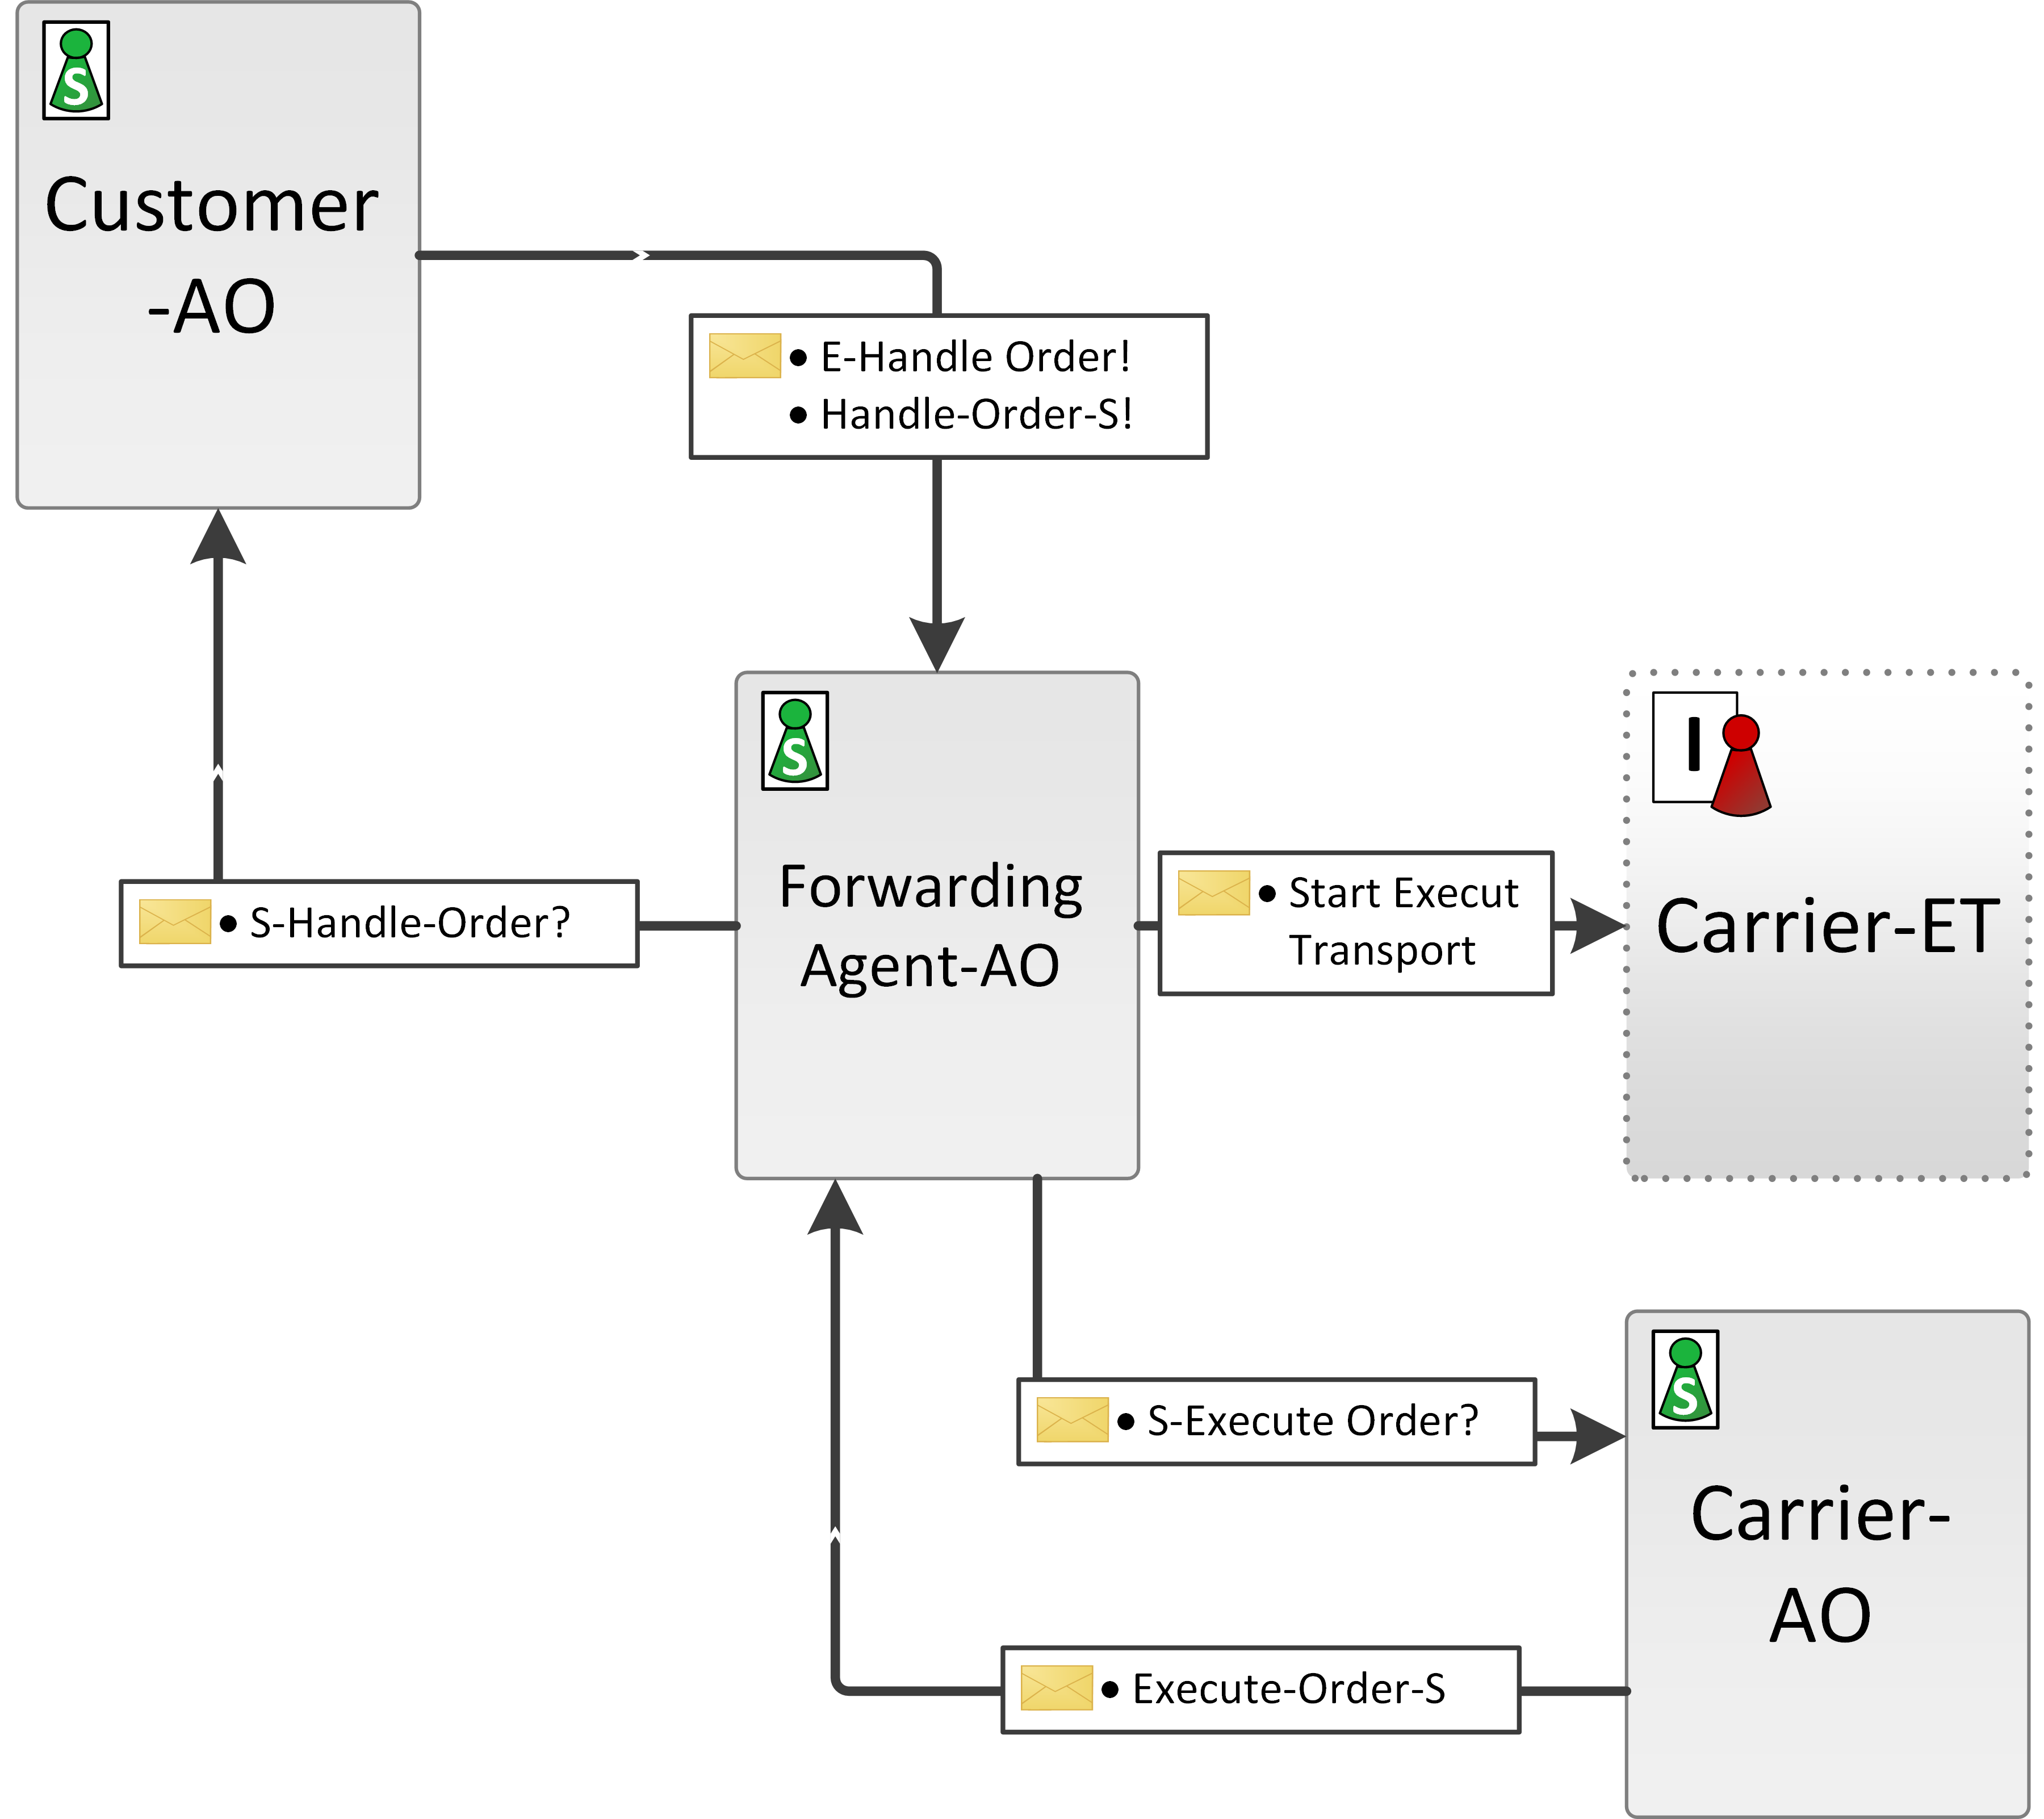
\includegraphics[scale=0.7]{Figures/Chapter5/Subject-Phase/SCD-Order_NEW.png}
	\caption{Subject Communication Diagram of S-PM of Process 'Order'}
	\label{fig:SCD-Order}
\end{figure}
\\
Subject 'Customer-AO' is the start subject. It is the only subject which executes activities in the start phase of the S-PM Order. The succeeding phase 'Handle order' is executed by subject 'Forwarding Agent' therefore subject 'Customer' sends the message 'E-handle-Order' to subject 'Forwarding agent-AO'. This subject executes the activities in phase 'Handle Order' (see figure \ref{fig:S-PM-Order}). \\
Figure \ref{fig:SBD-Customer-AO} shows the behavior of subject 'Customer-AO'. In order to see the relationship between the phases in the S-PM and the activities in the SBD the activities in the SBD belonging to certain phase in the S-PM have frames marked with the phase name.
\begin{figure}[hbtp]
     \begin{center}
	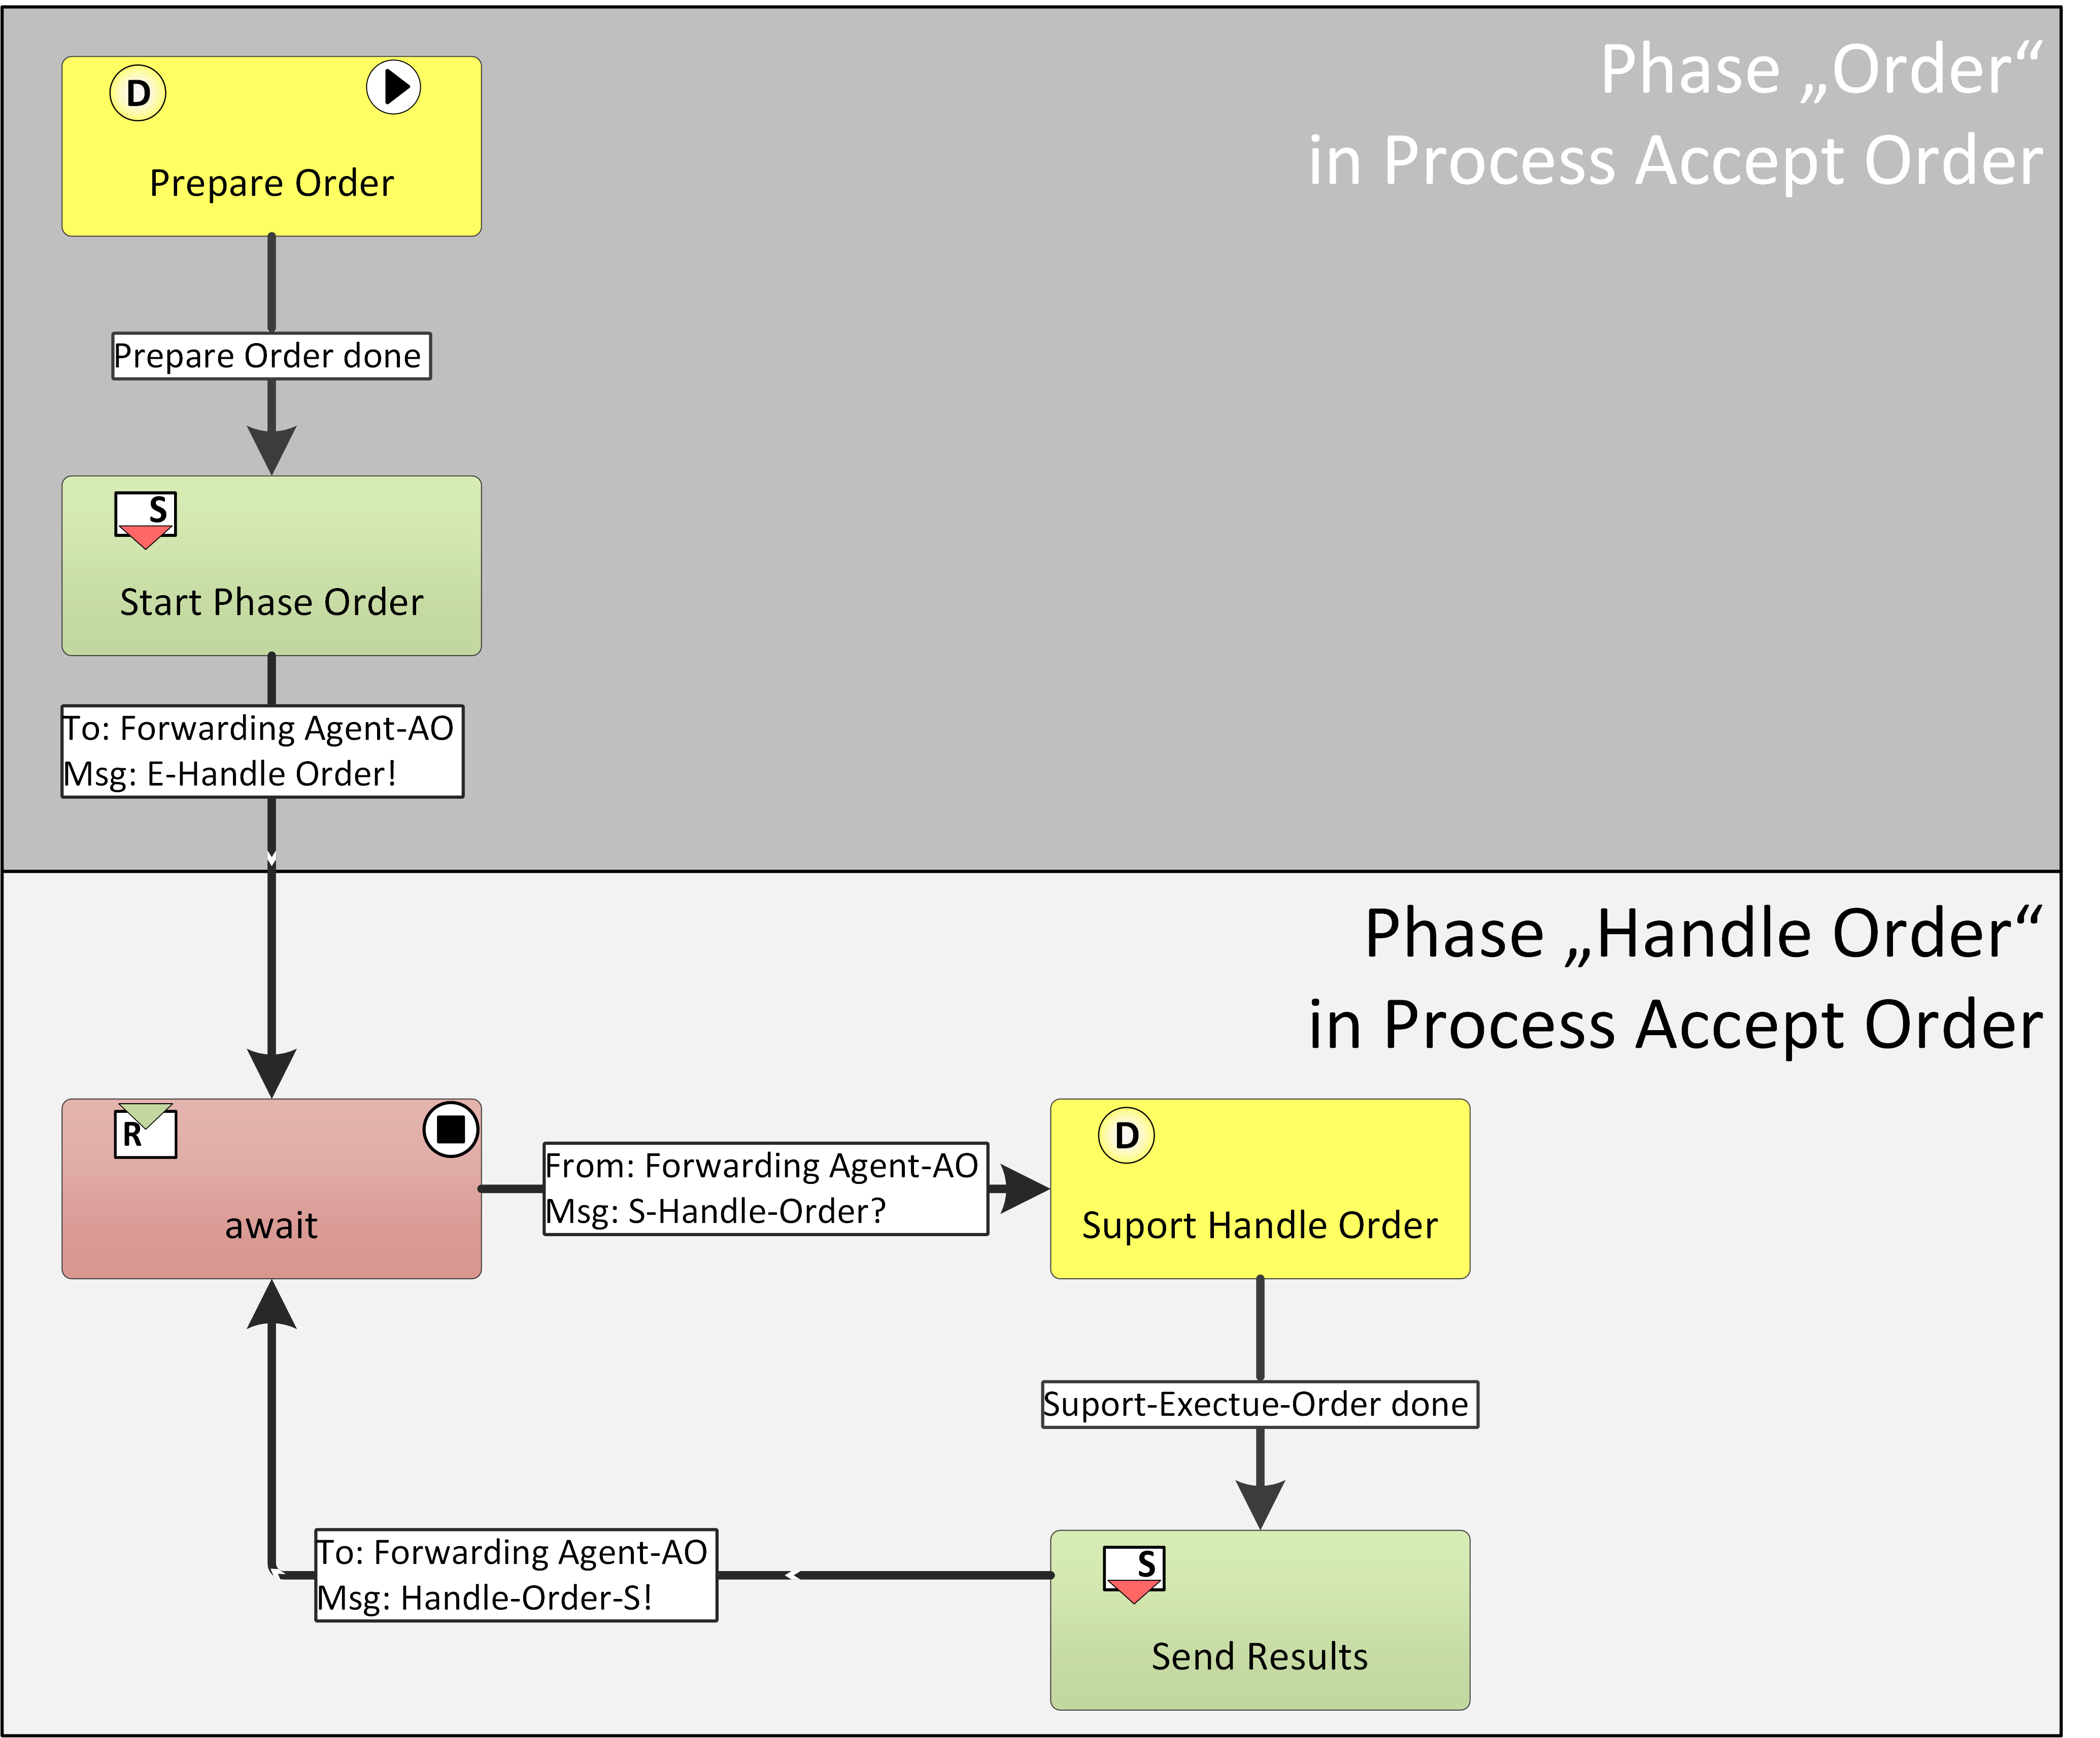
\includegraphics[width=0.6\textwidth]{Figures/Chapter5/Subject-Phase/SBD-Customer-AO_NEW.png}
	\caption{SBD of Subject 'Customer-AO'}
	\label{fig:SBD-Customer-AO}
	 \end{center}
\end{figure}
After the activity 'prepare order' is finished the next phase is started by sending the message 'E-Handle-Order' to the subject 'Forwarding Agent-AO'. Than subject 'Customer-AO' is waiting for the message 'S-Handle-Order?' from subject 'ForwardingAgent-AO'. This is a support request which is sent by subject 'ForwardingAgent-AO' in phase 'Handle order'. The support activity is executed and the result is sent back to subject 'ForwardingAgent-AO'.
The following figure \ref{fig:SBD-ForwardingAGentAO} shows the more complicate behavior of subject 'ForwardingAgent'. 
The subject 'ForwardingAgent-AO' receives the message 'E-Handle-Order' from the subject 'Customer-AO' in phase “Handle Order” in the S-PM. After that message the subject 'ForwardingAgent-AO'  checks whether it need some support from the subject 'Customer-AO'. If support is required a corresponding support request message ('S-Handle-Order?') is sent to the subject 'Customer-AO'. After an answer has been received the subject 'ForwardingAgent-AO' continues its work and checks whether some additional support is required or the activities in that phase can be finished. If that phase is finished the subject 'ForwardingAgent-AO' continues its work in phase 'Execute Order'. Because the subject 'ForwardingAgent-AO' is also the executing subject for phase 'Execute order' it is not necessary to send an E.message to the executing subject of the succeeding phase. In phase 'execute-orde' the subject 'ForwardingAgent-AO' starts also the process 'Execute-Transport' by sending the message 'E-Start-Execute-Process' to the subject 'Carrier-ET' which is a subject in process 'Execute Transport'.


\begin{figure}[hbtp]
 \begin{center}
	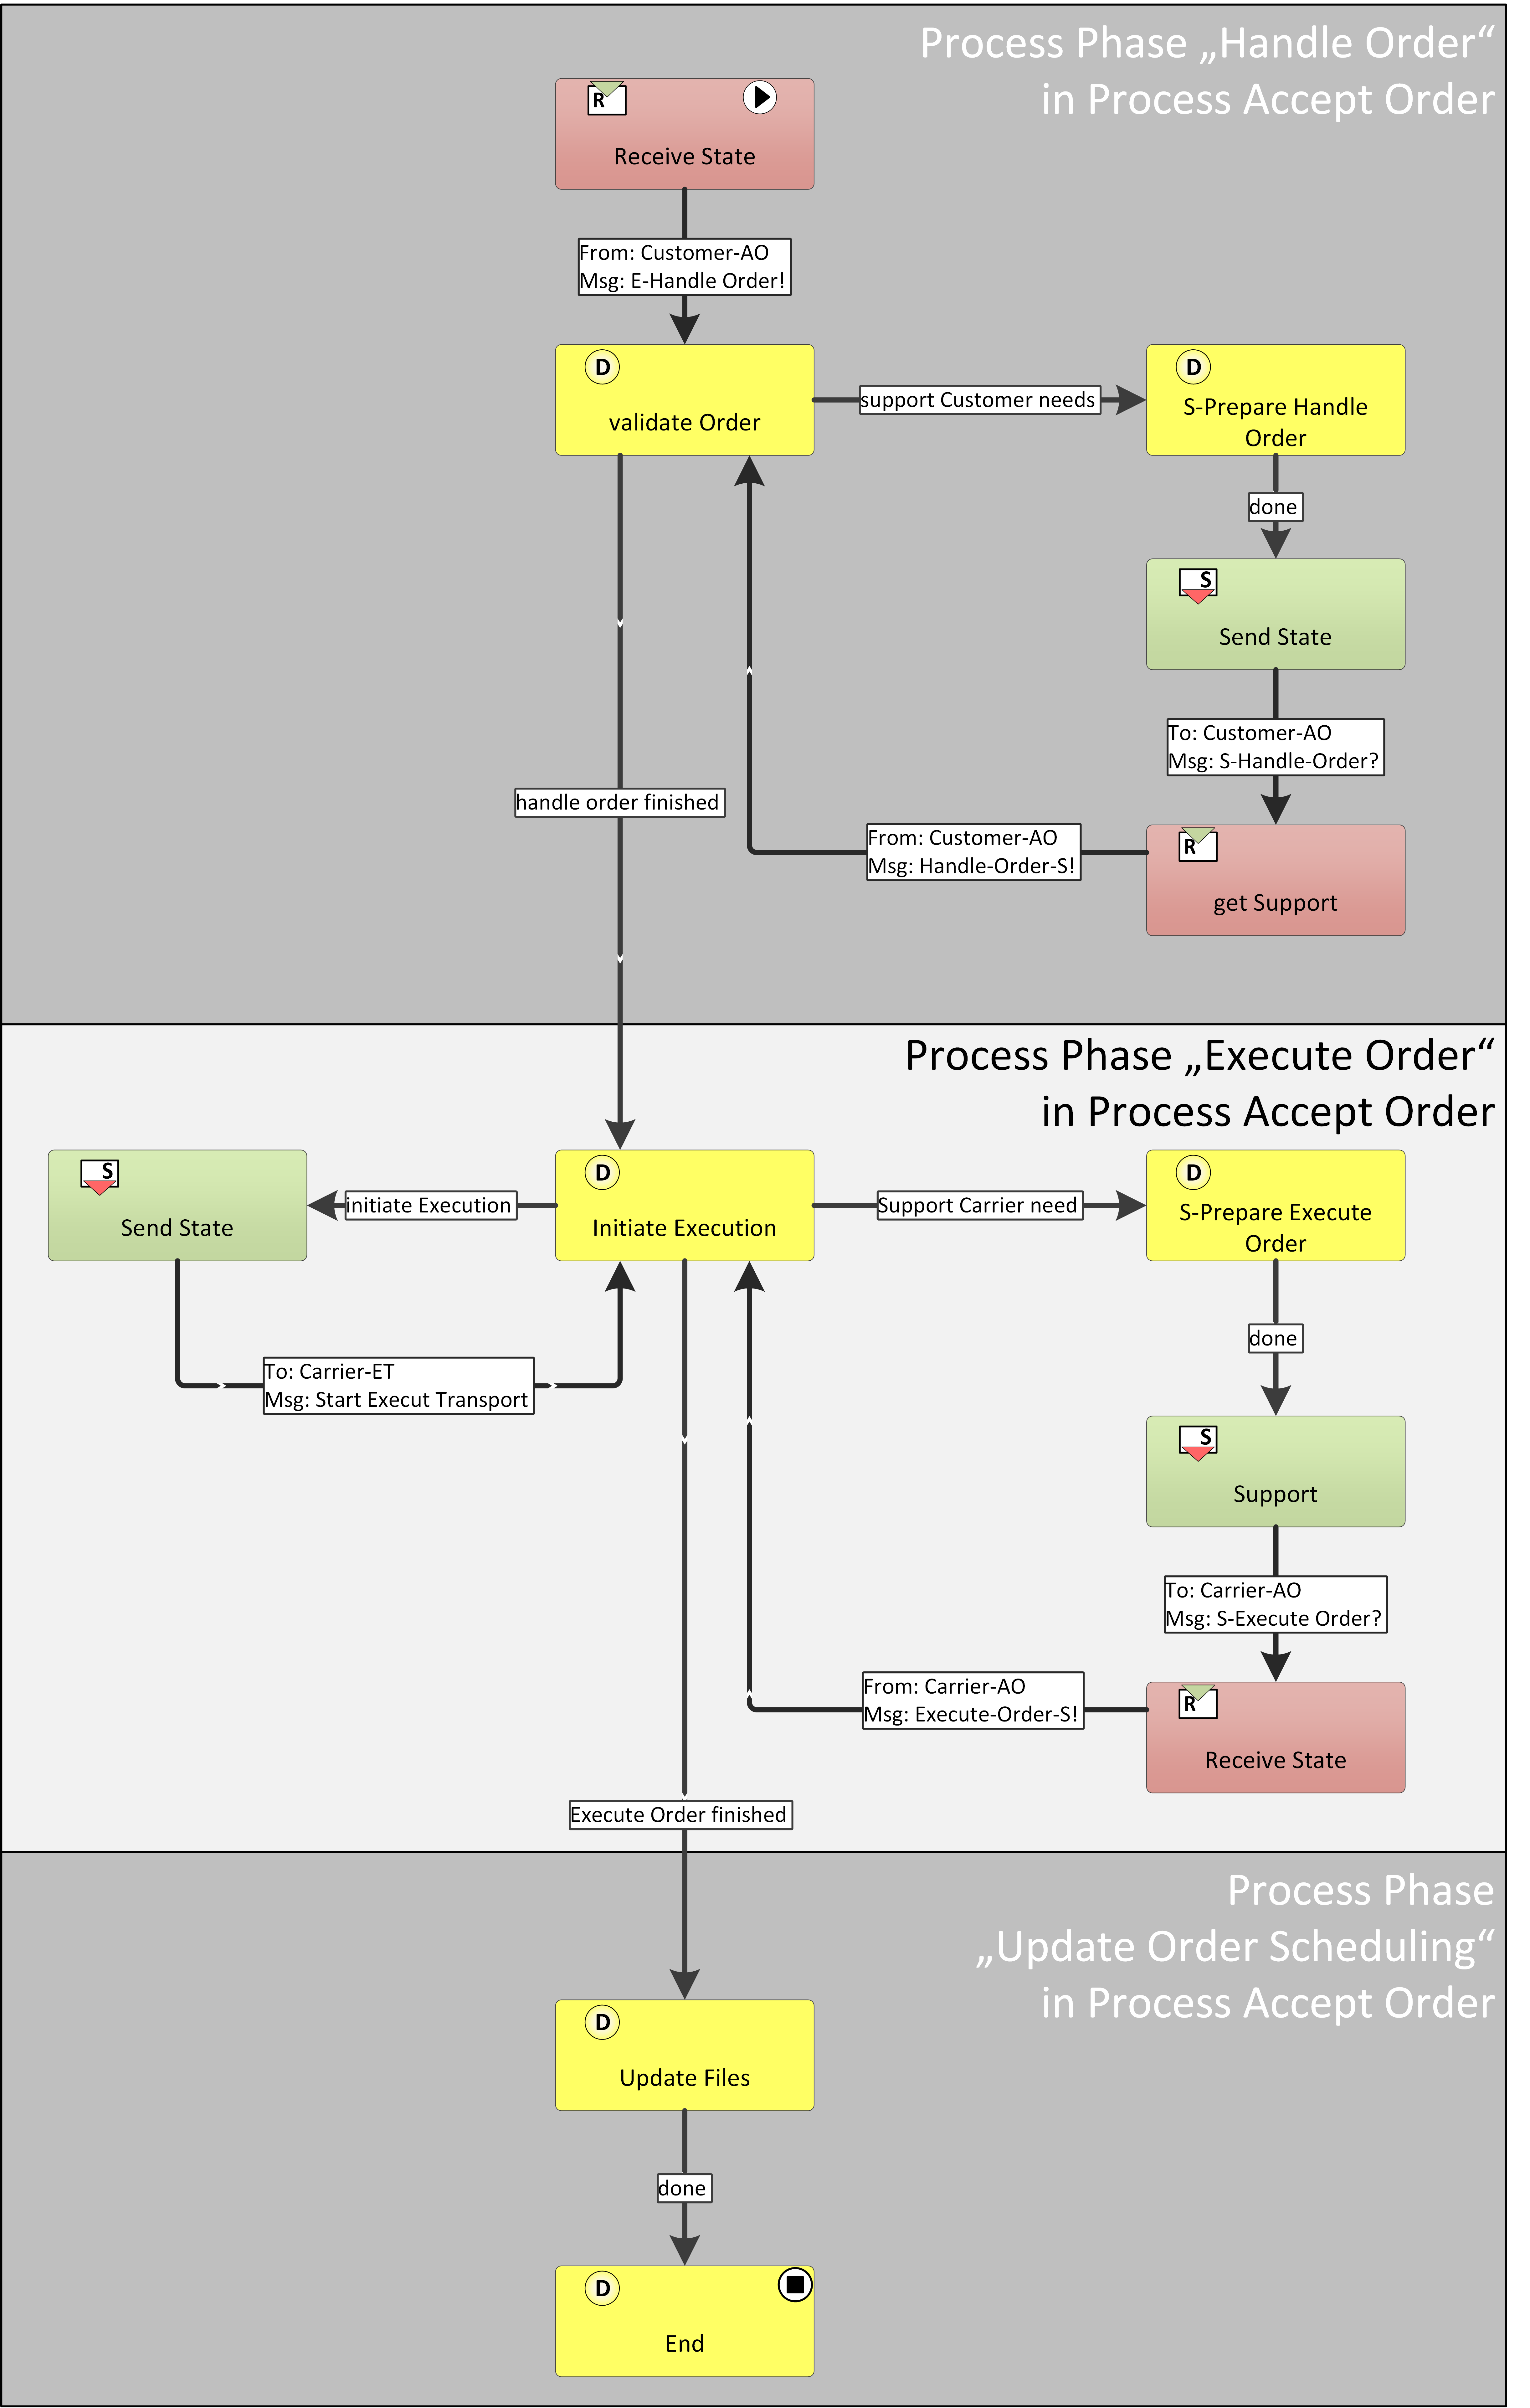
\includegraphics[width=0.9\textwidth]{Figures/Chapter5/Subject-Phase/SBD-ForwardingAGentAO_NEW.png}
	\caption{SBD of subject 'Forwarding-Agent' in Process 'Accept Order'}
	\label{fig:SBD-ForwardingAGentAO}
	\end{center}
\end{figure}


Figure \ref{fig:CarrierAO} shows the behavior of subject 'Carrier-AO'. In process 'Accept Order' the subject 'Carrier-AO' only supports subject 'ForwardinAgent-AO' in phase 'Execute Order'. This means the subject 'Carrier-AO' receives a support request message 'S-Execute-Order?', excutes the support activities and send the result back to the subject 'ForwardingAgent-AO' by the message 'S-Execute Order!'.

\begin{figure}[hbtp]
    \begin{center}
        
	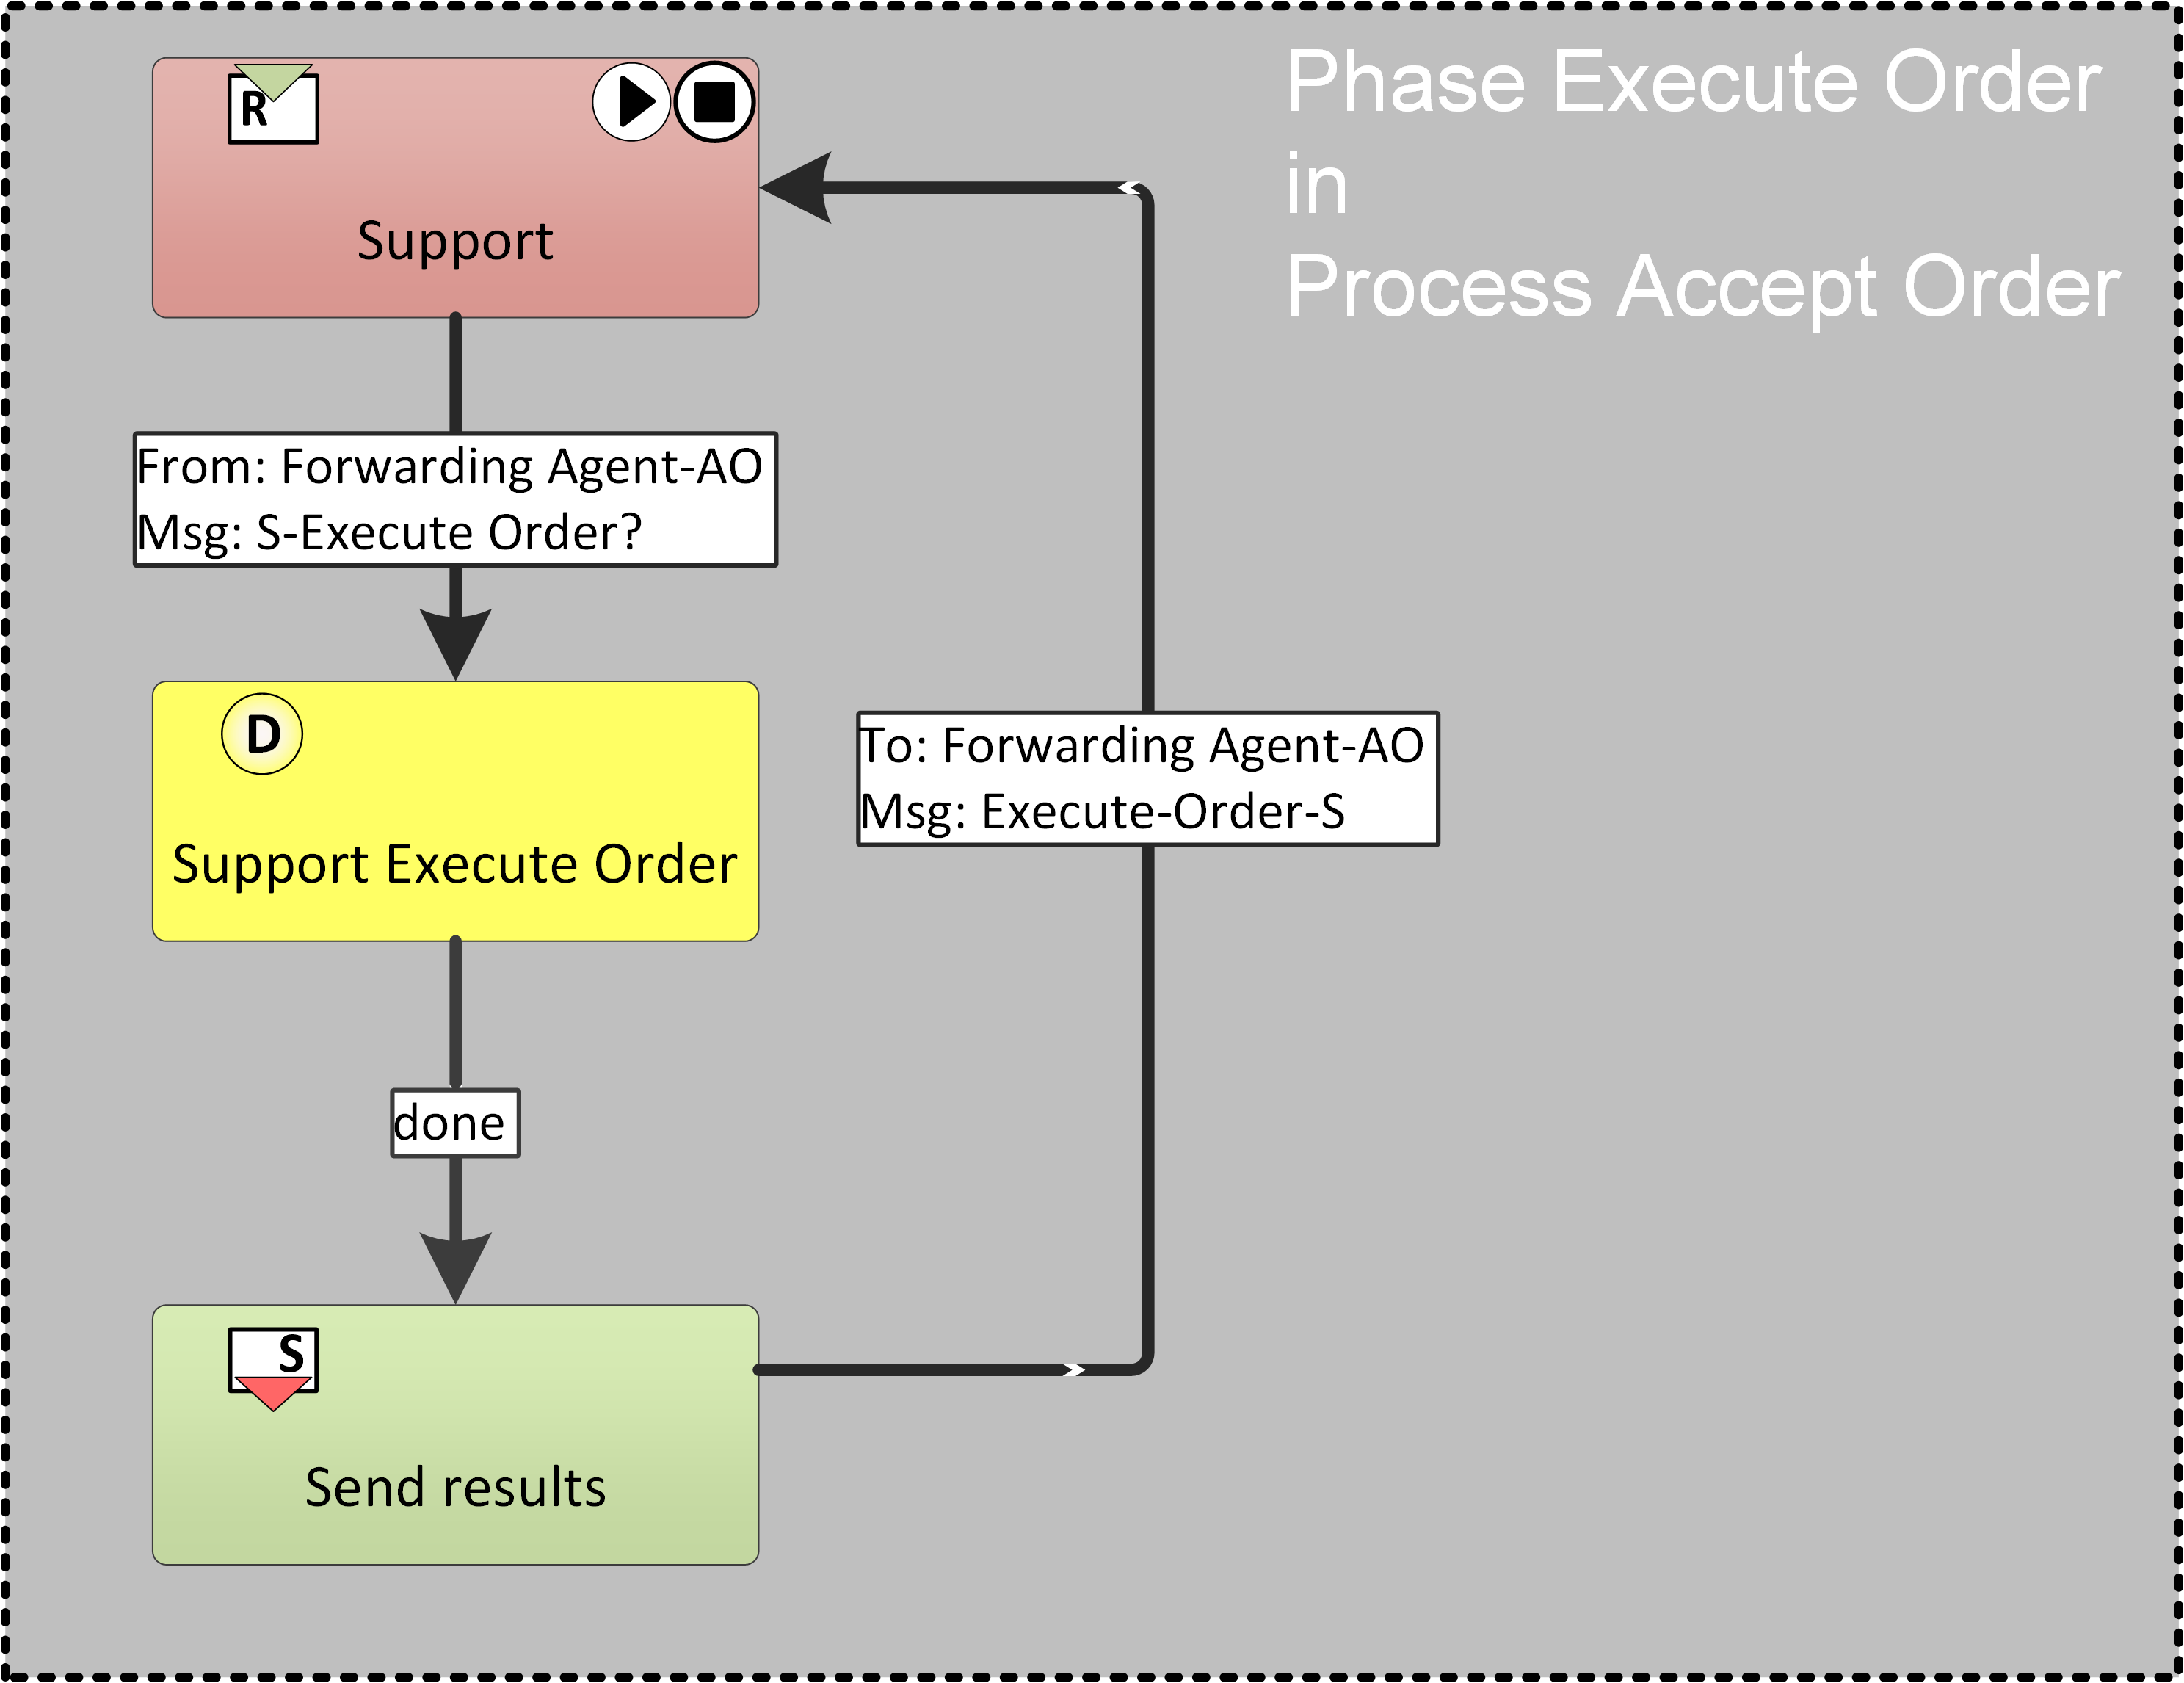
\includegraphics[width=0.5\textwidth]{Figures/Chapter5/Subject-Phase/CarrierAO_NEW.png}
	\caption{SBD of subject 'Carrier-AO' in Process 'Accept Order'}
	\label{fig:CarrierAO}
\end{center}
\end{figure}

Figure \ref{fig:SCD-ExecuteTransport} shows the SBD of process 'Execute Process' which is derived from the corresponding S-PM (see \ref{fig:S-PM-Execute-Trans}). The mechanism for getting the communication structure is the same as shown with process 'Accept Order'. The external subject 'ForwardingAgent-AO' represents the starting subject in process 'Accept-Order'.


\begin{figure}[hbtp]
	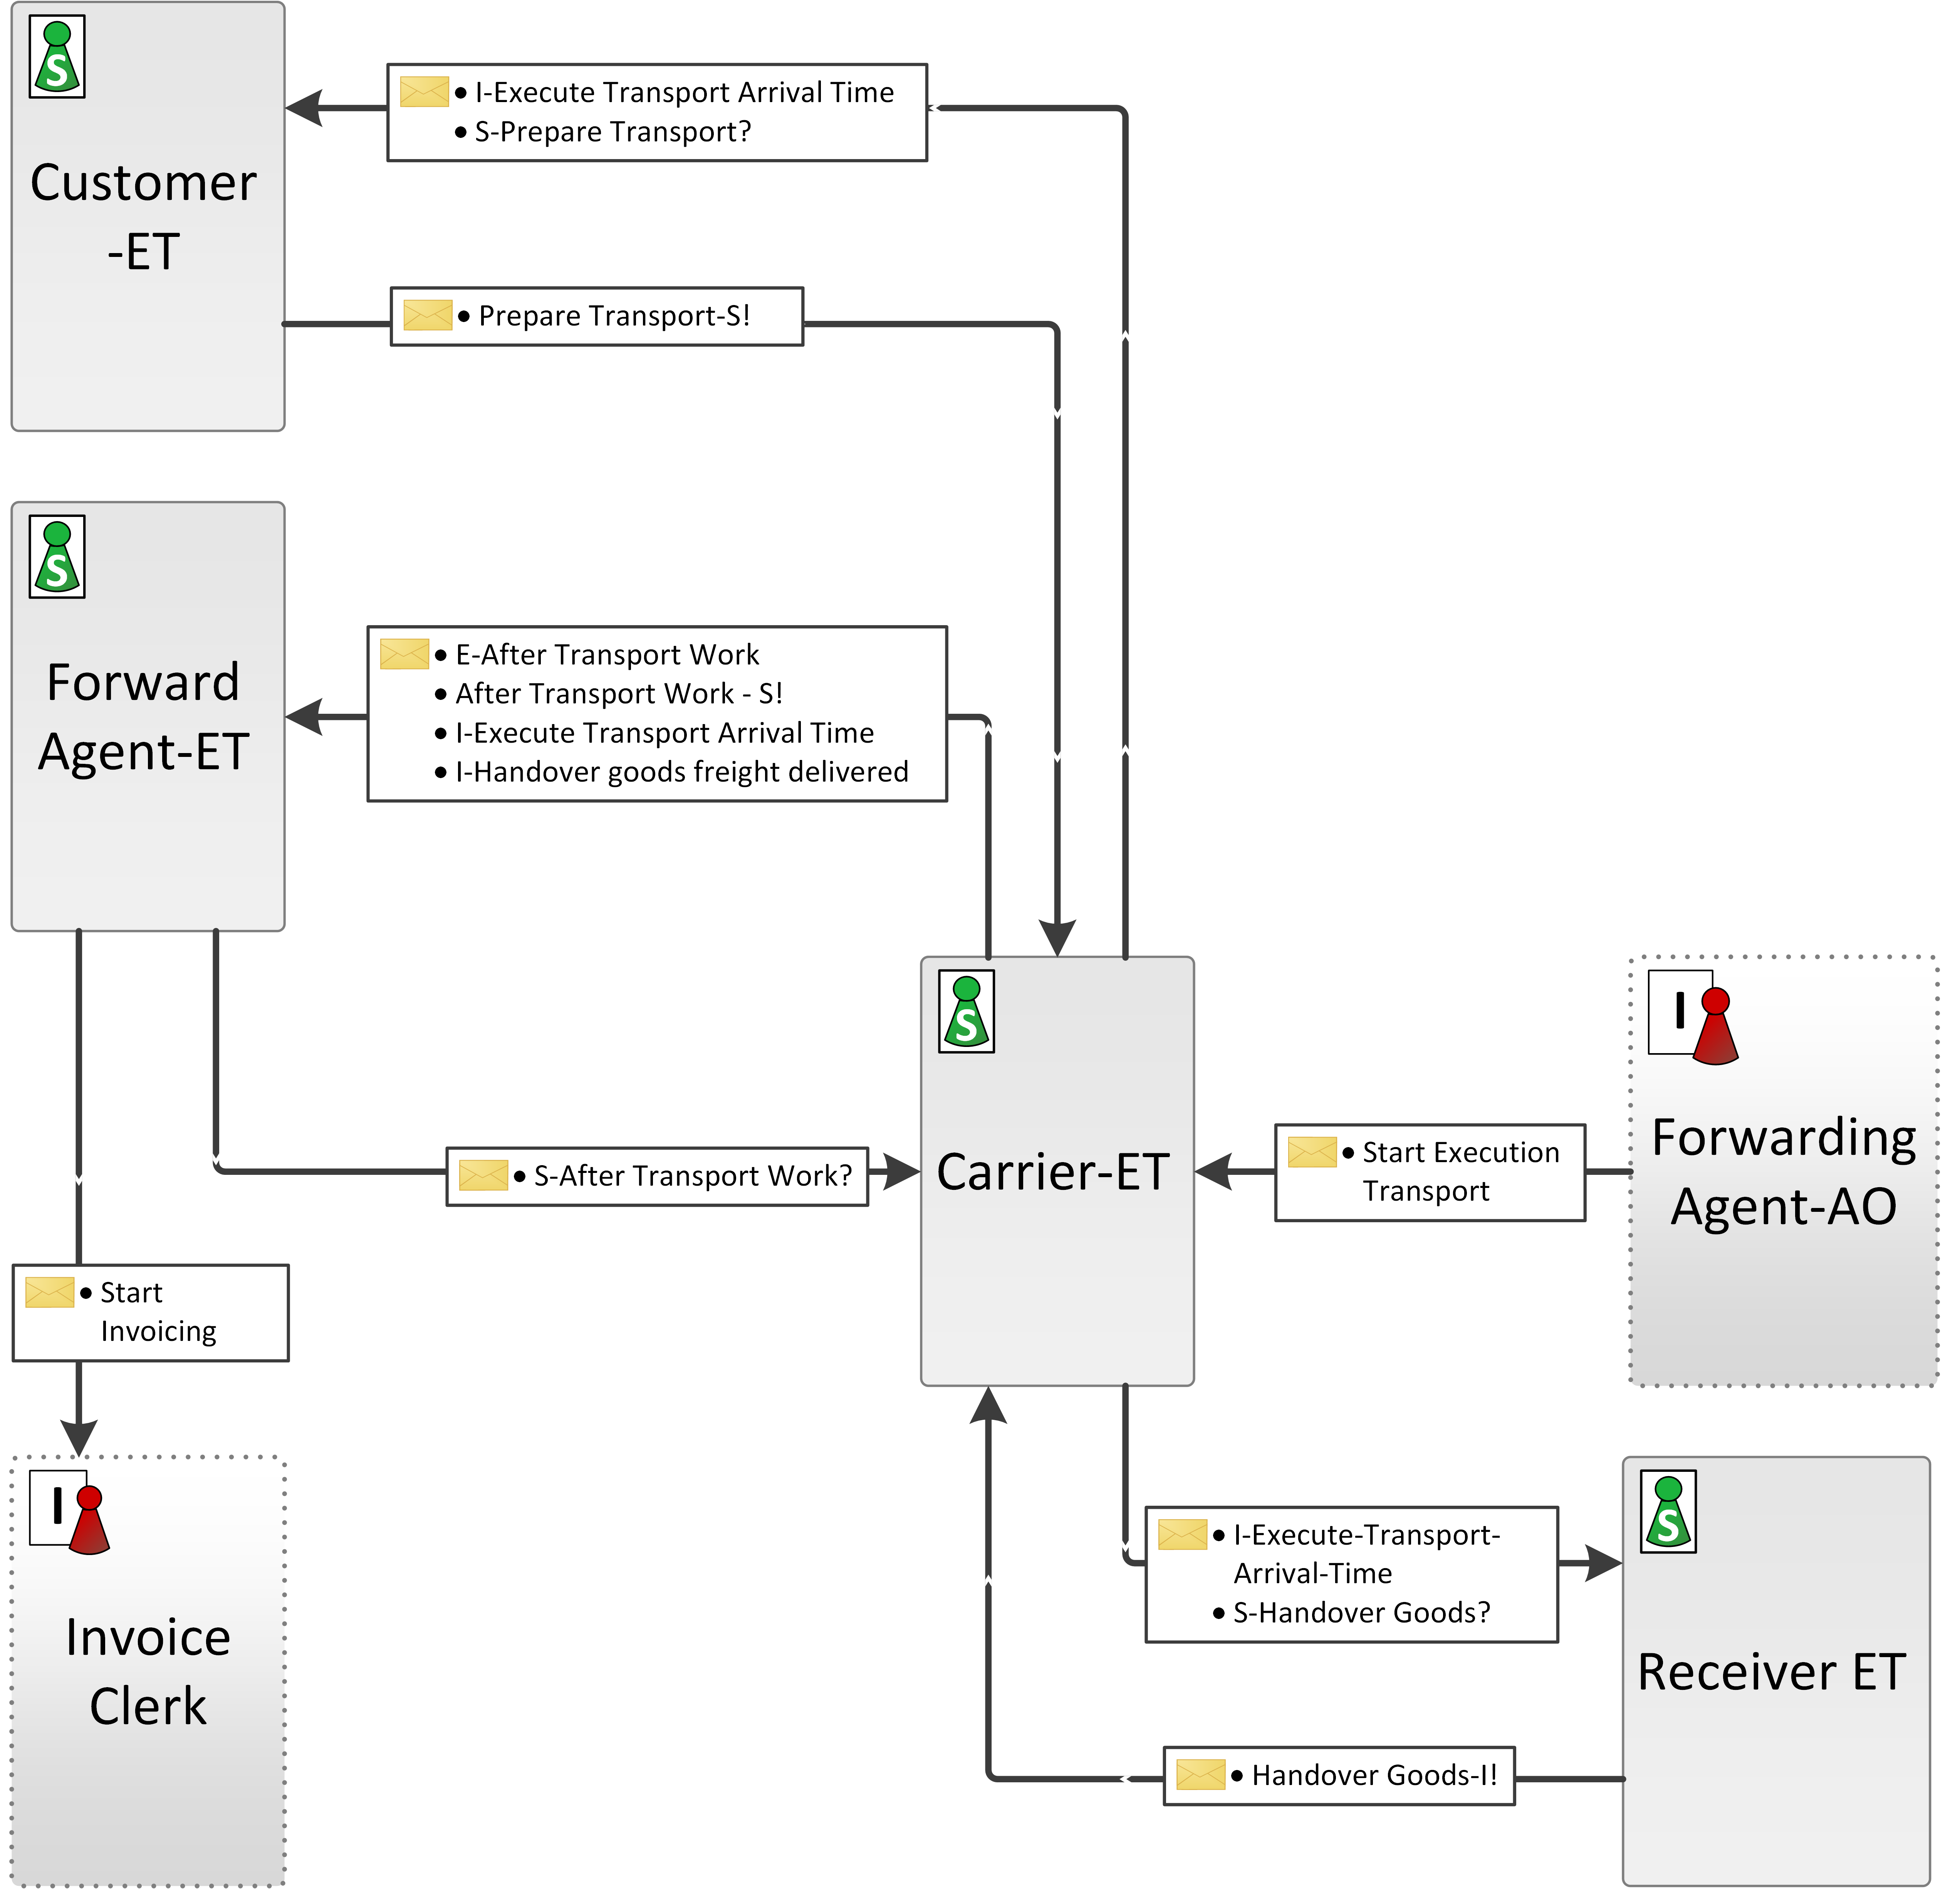
\includegraphics[width=0.9\textwidth]{Figures/Chapter5/Subject-Phase/SCD-ExecuteTransport_NEW.png}
	\caption{SID of Process 'Execute Transport'}
	\label{fig:SCD-ExecuteTransport}
\end{figure}

Figure \ref{fig:SBD-Carrier-ET} shows the behavior of subject 'Carrier-ET' for the first two phases of the corresponding S-PM shown in Figure \ref{fig:SBD-Carrier-ET}. This subject is different from the subject 'Carrier-AO' but it can be handled by the same person. But this is a decision during the embedding of a process into an organizational structure (see \cite{book:flei2011}).


\begin{figure}[hbtp]
	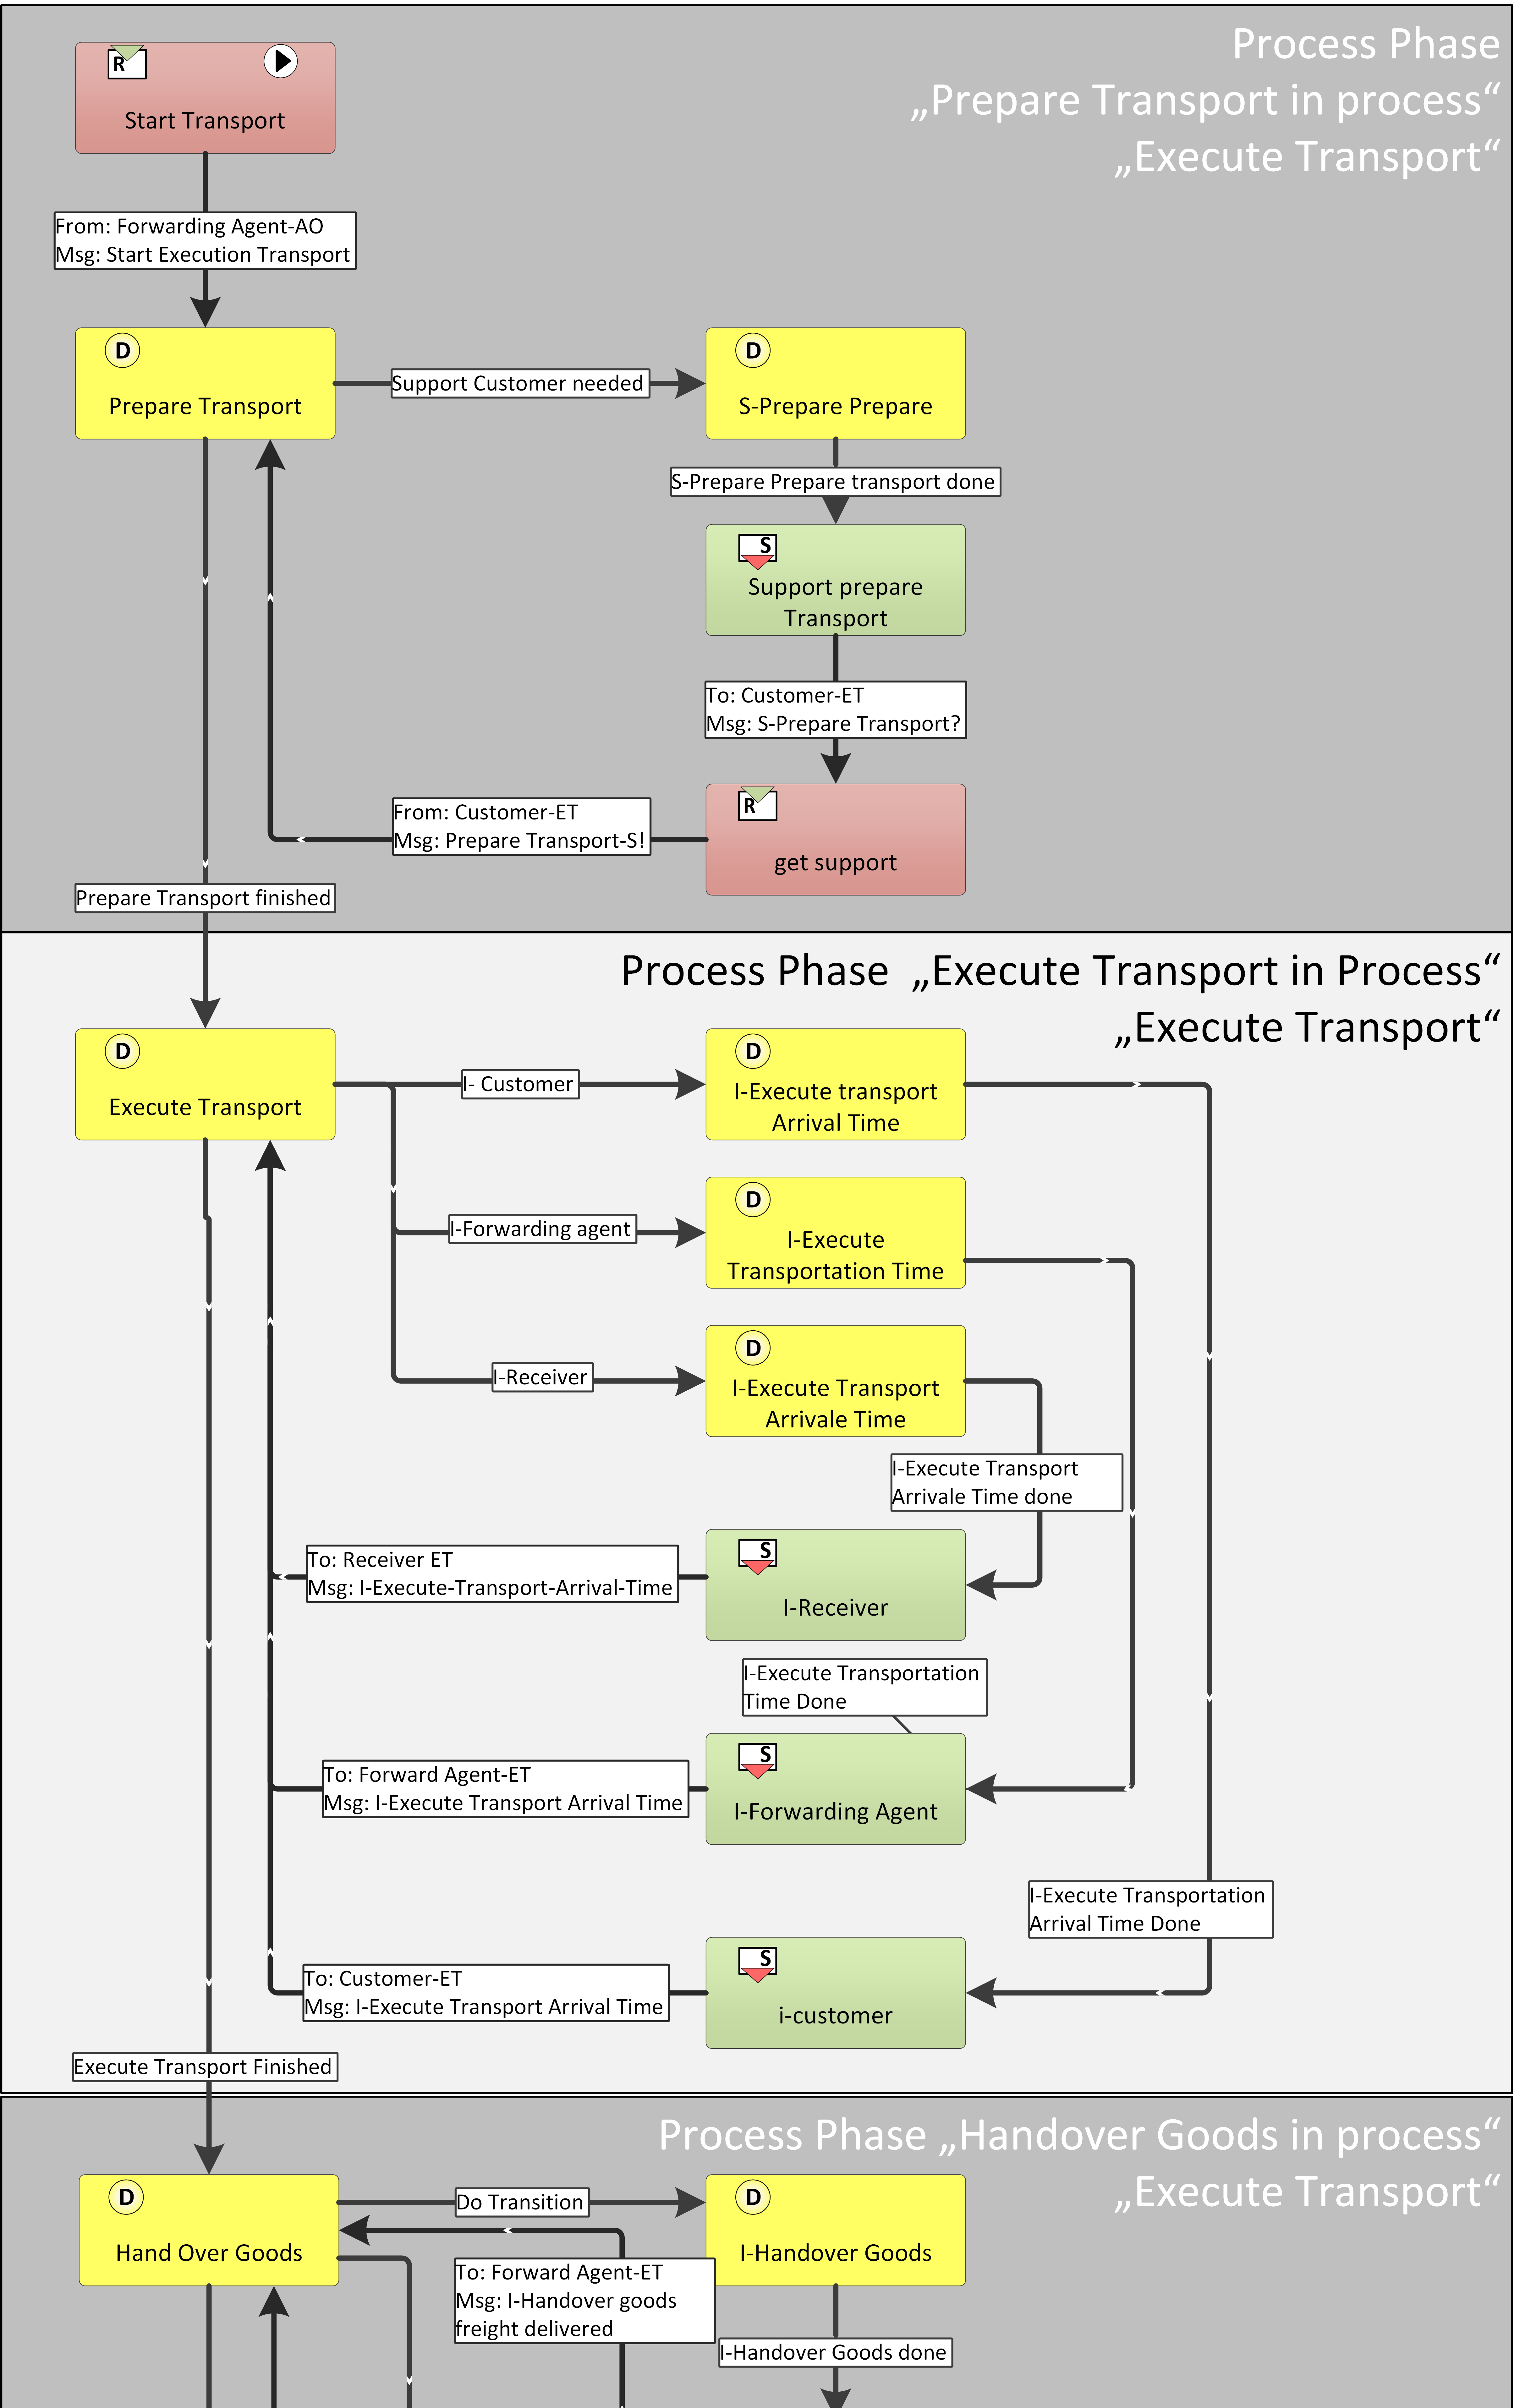
\includegraphics[scale=0.7]{Figures/Chapter5/Subject-Phase/SBD-Carrier-ET_NEW.png}
	\caption{SBD of Subject 'Carrier-ET' in Process 'Execute Transport'}
	\label{fig:SBD-Carrier-ET}
\end{figure}


\subsection{Evaluation of the Transformation}
S-PMs combine SCD and SBD. It show the subjects as active elements in a process, which subjects communicate with each other and which are the major phases of a process. \\

The phases can be seen as subprocesses producing some interim results. The author do not know a general proof that all processes can be structured in phases, but many widely used process specification methods use process phases (see section 'related work'). In his practical work the author hasn't yet found a process which could not structured in 3 to 6 phases, sometimes up to 8 phases (around two out of hundred).
\\
The conversion of each process phase into SCD and SBD is based on modeling by restriction (see chapter 6 in \cite{book:flei2011}). Modeling by restriction is executed in 5 steps:

\begin{itemize}
	\item Identify the number of subjects involved in a process,
	\item give these subjects names which describe their task in the process,
	\item remove not allowed communication paths between subjects,
	\item introduce process specific message names
	\item adapt communication behaviour to process requirements
\end{itemize}

An S-PM contains the information to execute the first 4 steps automatically for each process phase.In a phase the E-Subject communicates with the S- and I-subjects in a not very strict way. This means an E-Subject can request a service from a S-subject as often it wants, which may be not correct in the sense of the considered process. Finally an E-Subject decides whether a succeeding phase is started. This means a S-PM is converted in a process consisting of a chain of not very strictly defined subprocesses derived by modeling by restriction from the S-PM.


\subsection{Activity and Data Details in S-PM}
In S-PM mainly the sequencees of the execution of the major activities are considered.  In order to describe data and the details of the activities executed in a process phase a so called Input Execution Output table (IEO-Table) is used.  The following figure \ref{fig:Inpurt-Execution-Output} shows the IEO-table for the S-PM of the process 'Accept Order'.

\begin{figure}[hbtp]
	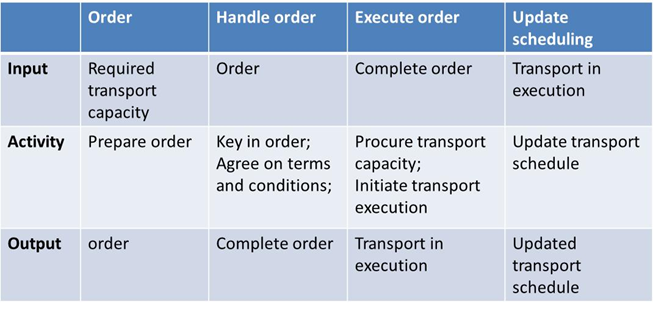
\includegraphics[scale=0.5]{Figures/Chapter5/Subject-Phase/Inpurt-Execution-Output.png}
	\caption{Input Execution Output Matrix of Process 'Accept Order'}
	\label{fig:Inpurt-Execution-Output}
\end{figure}

The columns represent the phases of a process as in the corresponding  S-PM. In the input row the data required in a process phase are specified, in the activity row the activities executed in a phase are listed and the output row contains the results of a process phase. 
The activities listed in the activity row define the details of the internal activity called 'phase name' or 'S-phase name' in a SBD derived from a S-PM. Based on that information the SBD can be described in more detail.
The input and output row can be used to define the business objects used by the various subjects and transported by the different messages.
In order to develop a systematic way to hand over that information to more detailed SCDs and SBD some additional work has to be done and experience has to be gathered. Up to now only a very intuitive approach is used.

\subsection{Conclusion}
S-PMs give managers and subjects involved in process an overview of a process provided that a process can be separated in phases. Practical experiences over more than 10 years show that this is possible without any difficulties. S-PMs are precisely defined which allows to convert them in SCDs and SBDs automatically. This conversion is based on modeling by restriction. This automatic conversion result in a first version of SCDs and SBDs which must be more restricted by the requirements of the considered process and enriched with the required business objects. Details for a S-PM are described in so called IEO-tables which contain details about the required data, the executed activities and the results of a process phase. In further work it has to be investigated how this infomation can be used in automatic conversions.

\subsection{Future Work}
Several aspects and topics need to be addressed by future research:
\begin{list}{-}{spacing}
	\item Definition of structural semantics in OWL
	\item Formal definition of the transformation from a Subject-Phase Matrix to a subject oriented model
\end{list}